\documentclass[11pt]{article}
\usepackage{graphicx}
\usepackage[top=35mm,
            bottom=25mm,
            left=20mm,
            right=20mm]{geometry}
%Gummi|063|=)
\title
{
  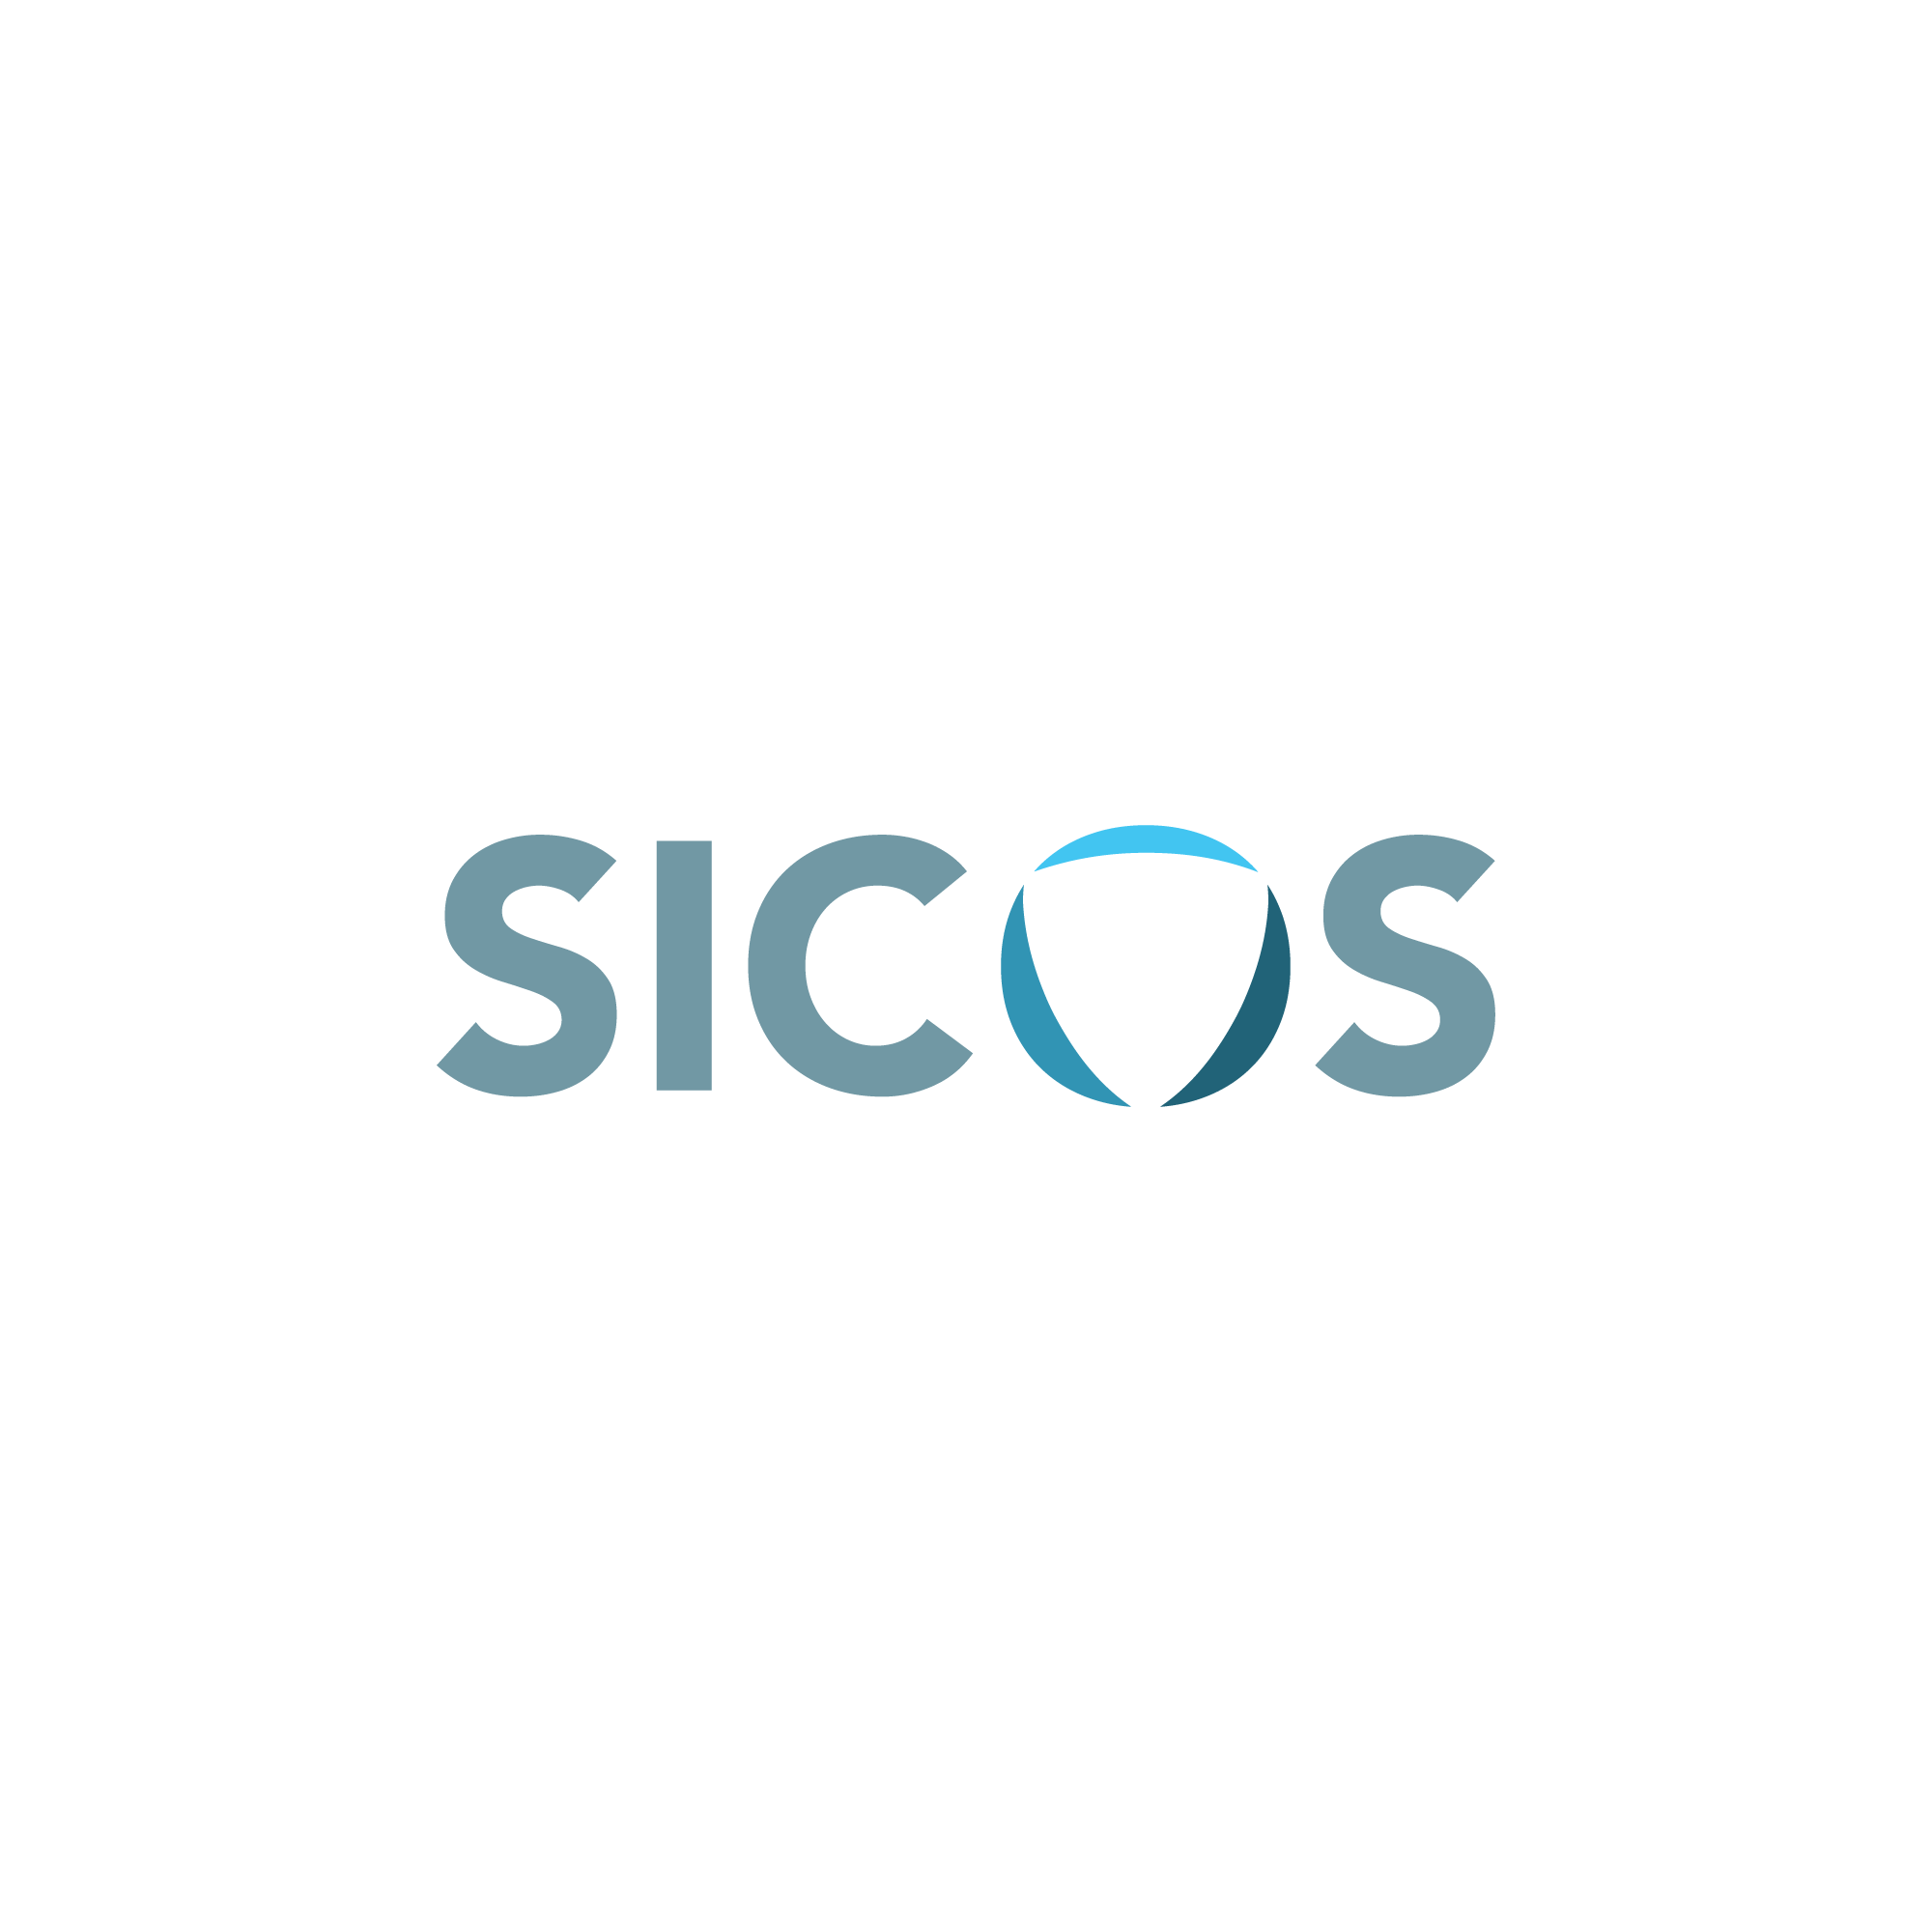
\includegraphics[scale=0.17]{sicos-logo2}      
  Technical specifications   
  of the SICOS platform
      }
\author{Lukas Cremer}
\date{9.8.2017}
\begin{document}
\maketitle
\newpage
\section{Goal}
The goal is, to provide a Platform where start-ups and SMEs can easily get funding for their business or project from investors, who register on the website. Accredited investors can buy tokens in an ICO and monitor or transfer their token holdings. 
The platform is helping start-ups to easily start their company, get all the paperwork done and get legal advice.  Start ups can initiate a token sale and monitor the status of their ICO.
The tokens issued on the platform will be a representation the companies profit. Each Token yields the Investor a fixed percentage of the companies profit. The dividends will be credited to the account of the investor. The tokens are KYC/AML compliant. Tokens can be bought  per bank wire transfer or alternative payment providers like Paypal. Tokens can be transferred between registered customers.  

\section{Harvest Token Platform}

The SICOS website is the platform were investors and companies can interact with the SICOS system. The site has four major parts. 
\subsection{Investor interface}
The investor interface will host all the services for investors on the site. To access all the functions provided by SICOS, investors have to register on the Platform. After registration investors can participate in token sales, create accounts, and monitor their assets. Tokens can be transfered to other registered investors on the website and any other function of the token contract can be called. The Website can also offer other functions on the Ethereum network, like creating new account, similar to other on-line wallets.

\subsection{Online Wallet}
Every investor needs an Ethereum address to interact with the token contract. This address can be generated on the website. Investors can also use their existing addresses to store the tokens. 
The Website includes an on line Wallet similar to myetherwallet.com . Investor can see their balances of different Tokens, transfer Tokens and initiate other functions of the smart contract. To initiate a call to any function investors have to provide their private key. The Wallet Software will then sign the transaction with this key and relay the signed transaction to an Ethereum node via an RPC interface. Investors can also use third party client software they trust, like the official Ethereum wallet to interact with the token contract.
The Online Wallet also allows the use of Hardware wallets like Nano ledger.

\subsection{Company interface}
On the company interface start-ups and SMEs can register to the SICOS platform. The registration process is checked manually by SICOS. Registered companies or projects can get consulting services from SICOS. In a later stage these services will be partially automated with templates that make the handling of the legal paperwork easier.
Companies can monitor the status of their Token sale on the website.
\subsection{Marketplace}

The marketplace provides information about the different companies that offer tokens on the platform. Investor can see upcoming ICOs, monitor the status of active Token sales and get information on projects that are already launched.

\section {Functions on the Platform}


\subsection{Registration process}
There will be two steps for the registration of investors on the Website. In the first step Investors will only provide their name an email address. After signing in, they have access to the investor interface and get  more detailed information on the marketplace. To participate in ICOs investors have to do a second registration process, that involves providing their ID and proof of address. An external provider of KYC-services will take care of registering the investor.  


\subsection{Key recovery}
There will be a key recovery process to allow investors who lost the private key of their account. This change in the token balance has to be verified by a trusted third party. This only applies to the tokens issues on the platform, not to other tokens or cryptocurrencies stored on the address. 


\subsection{Investor database}
The data of accredited investors acquired in the registration process will be stored in in an Investor database.
The investor database stores all personal information of all investors on the SICOS platform. The Investor database will be run by an external service provider or by SICOS itself. 


\subsection{Deleting Users}

Due to GDPR compliance user have to be able to delete themselves from the Investor database. This is only possible if the investor has no balance of any Token. When a investor wants to be deleted, a control server checks the Token balances of the user and only deletes the account after the balances are zero.

\subsection{Registry Control Server}

 The Ethereum address of the investors will be stored in a registry contract on the blockchain.

\subsection{Bank Control Server}
The control server is listening to all event on the bank account and calls the token contract as soon as an investment is coming into the account. Ideally the bank provides  some sort of authentication of investments made, that can be verified by the token contract. 
The control server is maintained by SICOS.


 \begin{figure}[ht]
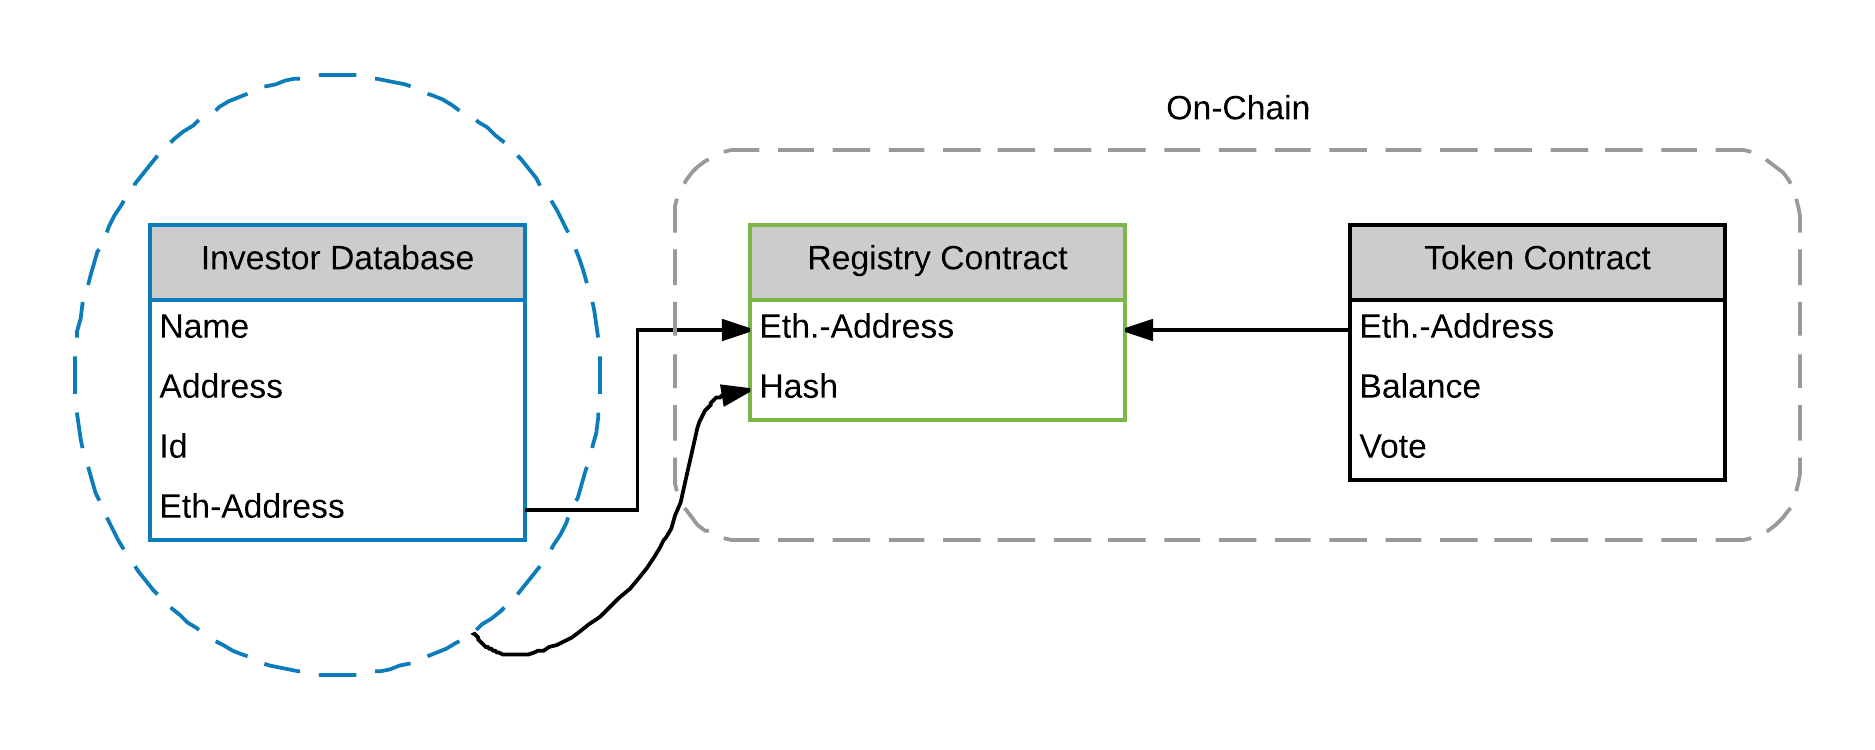
\includegraphics[scale=0.20]{Sicos-Base-Reg-Token.png}
\caption{Overview of the registration }    
\end{figure}[ht]  

\section{Smart Contracts}


\subsection{Registry Contract}

Only token holders whose ethereum addresses are registered in the registry contract can receive and send tokens. To secure the privacy of investors personal data, the registry is split into two parts. 
The registry contract is the representation of the Investor database on the blockchain. It stores the addresses of all Investors registered in the database. It also stores the hash of the database entry to ensure that the record in the database is not tampered with. Addresses can be added, changed and removed according to the rules set in the registry contract. 

\subsection{Harvest Token Contract}
The token contract is an ERC20 Token contract on the Ethereum blockchain, that manages Token issuance and transfer. Tokens of early investor can be looked in the contract during the ICO. Transfers of tokens are limited to addresses registered in the registry contract. The token contract defines the rules under which tokens are issued and transfered. It will make sure that only registered investors are able to hold tokens. 
Investors can use any Ethereum wallet to interact with the token contract.
The Token contract has a function where the dividend of the company can be reported to the contract. This dividend will then be distributed to all token holders. The dividend will be updated with every interaction with the token contract. 

\subsection{Euro Token}
The Euro Token stores the investors balances denominated in Euro. It will be managed by SICOS. The token contracts can mint new Euro-Token in case of a dividend distribution. Investors can redeem their Euro-Token via the platform. Euro-Tokens are not transferable but to SICOS. 
The Bank control server will look up which investors want their tokens redeemed and will transfer the Euros to the investors.
 


\begin{figure}
\begin{center}
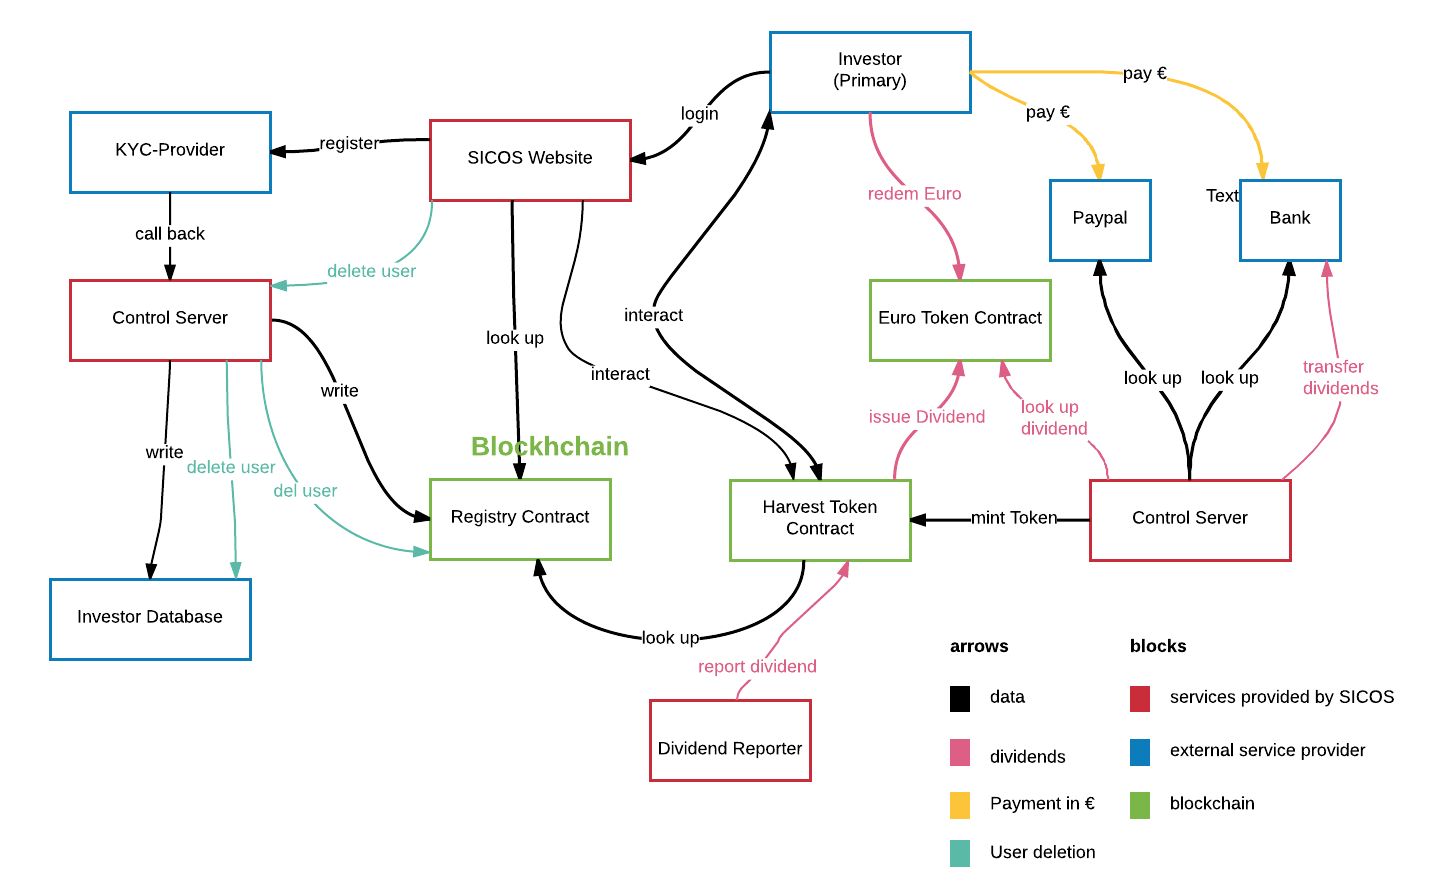
\includegraphics[scale=0.38]{sicos-diagram2.png}    
\end{center}
\end{figure}

 
\subsection{Contract Auditing}
SICOS will provide a template for the Token contract for an ICO, this contract will be externally audited by different smart contract auditing providers. 
Every Token sale on the SICOS platform will have their own token contract, If any changes made to the already audited contract, these changes have to be externally audited too.
 
\section{External service providers}

\subsection{ KYC provider}
The KYC provider needs to be fully compliant with KYC regulation of the jurisdiction.

\subsection{Account information Provider}
The Investor data base is run by a account information provider, that stores all personal data of the investors. This service provider gets the personal investor information directly from the video identification provider. The account information provider has to comply with the EU-General Data Protection Regulation. This role is either done by the the KYC Provider or SICOS itself

\subsection{Bank}
The Company doing the ICO with SICOS has to have a bank account with the partner bank. The partner bank accepts money from investors and deposits it to the account of the company. 
Investors can transfer money to the bank account. The control server watches the incoming payment on the bank account via an API, and issues tokens corresponding to the investment made.

\subsection{Payment Provider (e.g. Paypal}
Investor can also pay via an Payment provider like Paypal. The control server also fetches the in coming transfers via an API and sends a message to the token contract to mint new token.

\subsection{Exchanges}
For cryptocurrency exchanges to be able to list the tokens issued on the SICOS platform on a secondary market, they have to integrate the registry into their existing trading system. In a later stage accredited exchanges can have access to write their own customers into the registry contract when they provide the investors data to the investor database. 

\end{document}
\grid